\documentclass{tufte-handout}

\title{GGSB 2015 Prelim} %\thanks{Inspired by Edward~R. Tufte!}}

\author[The Tufte-LaTeX Developers]{Charles Czysz}

\date{September 2015} % without \date command, current date is supplied

\setcounter{tocdepth}{3}

\geometry{bottom=0.5in}%showframe % display margins for debugging page layout

\usepackage{hyperref}
\hypersetup{
  colorlinks   = true,    % Colours links instead of ugly boxes
  urlcolor     = blue,    % Colour for external hyperlinks
  linkcolor    = black,    % Colour of internal links
  citecolor    = red      % Colour of citations
}
\usepackage{graphicx} % allow embedded images
  %\setkeys{Gin}{width=\linewidth,totalheight=\textheight,keepaspectratio}
  \graphicspath{{./figs}} % set of paths to search for images
\usepackage{amsmath}  % extended mathematics
%\usepackage{float}
\usepackage{booktabs} % book-quality tables
\usepackage{units}    % non-stacked fractions and better unit spacing
\usepackage{multicol} % multiple column layout facilities
\usepackage{lipsum}   % filler text
\usepackage{fancyvrb} % extended verbatim environments
\usepackage{amsthm}
  \fvset{fontsize=\normalsize}% default font size for fancy-verbatim environments

% Standardize command font styles and environments
\newcommand{\doccmd}[1]{\texttt{\textbackslash#1}}% command name -- adds backslash automatically
\newcommand{\docopt}[1]{\ensuremath{\langle}\textrm{\textit{#1}}\ensuremath{\rangle}}% optional command argument
\newcommand{\docarg}[1]{\textrm{\textit{#1}}}% (required) command argument
\newcommand{\docenv}[1]{\textsf{#1}}% environment name
\newcommand{\docpkg}[1]{\texttt{#1}}% package name
\newcommand{\doccls}[1]{\texttt{#1}}% document class name
\newcommand{\docclsopt}[1]{\texttt{#1}}% document class option name
\newenvironment{docspec}{\begin{quote}\noindent}{\end{quote}}% command specification environment

\newtheoremstyle{noparens}%
{}{}%
{\itshape}{}%
{\bfseries}{ - }%
{ }%
{\thmname{#1}\thmnumber{ #2}\thmnote{ #3}}

\theoremstyle{noparens}
\newtheorem*{define}{Definition}
\newtheorem*{example}{Example}

% Normal font formatting for subsections (i.e. questions)
\titleformat{\subsection}
{\large\bfseries}{\thesection}{1em}{}
%\normalfont
\usepackage{makeidx}
\makeindex


\begin{document}

\maketitle% this prints the handout title, author, and date

\noindent
\textbf{Required}

1-8: General Genetic Principles

9-12: Mapping

39-50: Study Design and Statistical Data Analysis

\vspace*{1\baselineskip}

\noindent
\textbf{Choice between}

13-17: Genetic Architecture of Human Phenotypes

\noindent
\textbf{or}

18-28: Population and Evolutionary Genetics

\vspace*{1\baselineskip}

29-32: Molecular Mechanisms and Model Organisms in Human Genetics

\noindent
\textbf{or}

33-38: Gene Regulation and Human Phenotypes

\vspace*{4\baselineskip}
\begin{abstract}
\noindent
A good answer would show in escalating order: 
\begin{itemize}
\item Basic understanding via descriptions and definition of basic terms and concepts 
\item Knowledge of biology/literature via empirical examples of concepts in action, 
\item Engagement of critical thinking by highlighting well-known limitations or novel critiques of a concept or its common application 
\item Recognition of open problems and novel research opportunities.
\end{itemize}

\end{abstract}

\newpage

\tableofcontents 

\newpage
%\printclassoptions
 
\section{General Genetic Principles}\label{sec:gen-genetic}

\subsection{1.
Explain the distinction between allelic heterogeneity, genetic (locus) heterogeneity, and clinical heterogeneity. Give examples of each.}  
%\label{subsec:01}

\begin{abstract}
Great review of this topic:

\href{http://www.sciencedirect.com/science/article/pii/S009286741000320X}{Genetic Heterogeneity in Human Diseases}
\end{abstract}
%This question asks to explain how similar or identical phenotypes can have different underlying causes.

\noindent
\textbf{Overview}

\noindent
Each of the following topics have implications in the type of studies which can or cannot be used. Overall, heterogeneity ensures that large-scale association tests or case-control studies will be poorly powered to detect causal variants or genes. See the review linked above for more detail.

%\define[Allelic heterogeneity]
\begin{define}[Allelic Heterogeneity]
In a given population, different mutations in the same gene result in a similar phenotype.
\end{define}
\noindent
\textbf{Example} 

Cystic Fibrosis is caused by defective cystic fibrosis transmembrane conductance regulator proteins (CFTR). Many mutations in the CFTR gene can give rise to non-functioning proteins, which all lead to the same CF phenotype.

Two-thirds of all CF mutations are a 3bp deletion at position 508, resulting in a loss of phenylalanine. 1,500 other mutations also exist which lead to CF. However, this disease is haplosufficient..

Unknown alleleic heterogeneity can affect GWA results\footnote{\url{http://hmg.oxfordjournals.org/content/11/20/2417.short}} when LD methods are used.

\textbf{Sources}

\url{http://hmg.oxfordjournals.org/content/20/20/4082.short}

\begin{define}[Genetic (locus) heterogeneity]
Mutations in different genes result in a similar phenotype.
\end{define}

\begin{example}
The BRCA1 and BRCA2 genes are a good example of how mutations in different genes lead to the same phenotype. 
\end{example}

\begin{define}[Clinical Heterogeneity]
Variability in clinical manifestations, or phenotypes, with the same underlying mutation/genetic disorder.
\end{define}

Mutations in several genes can lead to familial hypercholesterolemia, high level of LDL cholesterol. Mutations in LDLR (LDL receptor), Apolipoprotein B, proprotein convertase subtilisin/kexin type 9 (PCSK9), and the ARH/LDLRAP1 genes can all lead to familial hypercholesterolemia.

\newpage
\subsection{2.
What is the relationship between the inbreeding coefficient, kinship coefficient, and coefficient of relatedness? How are they calculated in pedigrees? Can they be estimated in the absence of pedigree information?}
\label{subsec:02} 

\begin{define}[Identity by descent]
Two alleles at the same locus that are descended from the same ancestral allele within the recent past. Can be 0, 1, or 2 depending on how many ancestral alleles shared between individuals.
\end{define}

\begin{marginfigure}%
  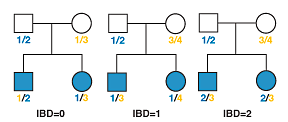
\includegraphics[scale=0.65]{./figs/ibd}
  \caption{IBD Pedigree Example}
  \label{fig:marginfig}
\end{marginfigure}

\begin{define}[Coefficient of Kinship]
$f_{xy}$: The probability that two alleles, one from X and the other from Y, are IBD.
\end{define}

\begin{figure}
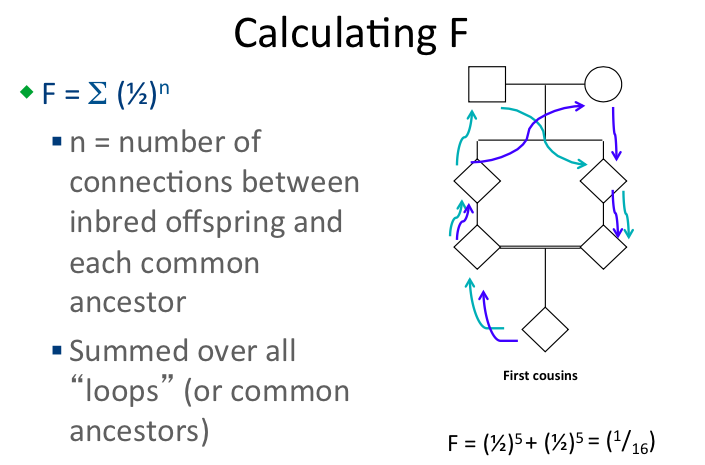
\includegraphics[scale=0.5]{./figs/kincoeff}
\end{figure}

\begin{define}[Coefficient of Relatedness]
$R_n$, the probability of sharing $n \in \{0,1,2\}$ IBD alleles. Mean relatedness, $\bar{r} = 0 \times r_0 + 1 \times r_1 + 2 \times r_2$.
\end{define}

\noindent
\textbf{Relationship between Coefficients}
\[f_{xy} = \frac{1}{2}\bar{r}\]
\begin{figure}[h!]
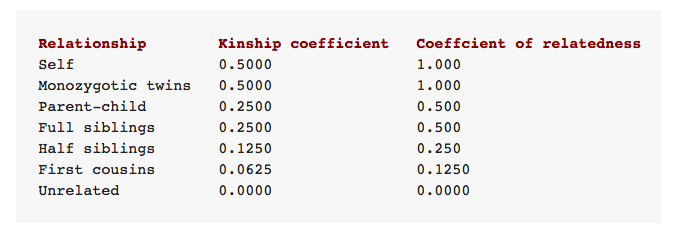
\includegraphics[scale=0.5]{./figs/kinrelate}
\caption{Relationship between Kinship and Relatedness coefficients}
\end{figure}


\newpage
\subsection{3.
What are the key distinguishing characteristics of pedigrees segregating autosomal dominant, autosomal recessive, X-linked, Y-linked, and mitochondrial diseases?}
\label{subsec:03}

 \noindent
 \textbf{Autosomal Dominant}
 
 On average, half of offspring of affected-nonaffected parents will be affected.
 
 \noindent
 \textbf{Autosomal Recessive}
 
 If both parents are carriers, then $\frac{1}{4}$th of offspring will show a disease phenotype.
 
 \noindent
 \textbf{X-linked Dominant}
 
Affected men always pass disease to daughters. Affected women have $\frac{3}{4}$ths chance of passing disease to daughters and same chance to sons.
 
 \noindent
 \textbf{X-linked Recessive}
 
Women can be either affected or carriers. Men always affected.
  
\newpage
\subsection{4.
Explain the "non-Mendelian" concepts of uniparental disomy and imprinting. How would these be manifested in pedigrees and how are they demonstrated at the cellular or molecular levels?}
\label{subsec:04}

\begin{define}[Mendelian Genetics]
Involves the "Laws" of random segregation, independent assortment, and dominance. Non-Mendelian genetics violate at least one of these assumptions.
\end{define}

\begin{define}[Uniparental Disomy]
Offspring inherits a chromosome, or part of one chromosome, from one parent only. These offspring are euploid, but with an unequal contribution of genetic material from the parents.
\end{define}

Uniparental disomy can manifest in two ways: inheriting both homologs from one parent (heterodisomy), or duplication of a single inherited chromosome (isodisomy).

\textbf{Heterodisomy}

Offspring inherits homologs from one parent only. Can occur during a nondisjunction error in Meiosis I, where one daughter cell inherits both sister chromatids while the other inherits none. This will lead to trisomy after fertilization, and heterodisomy if trisomy rescue occurs and results in the loss of the allele from the other parent.

Heterodisomy can also result from crossover events. In the parental generation, a cross between a balanced translocation carrier and a normal carrier can result in partial heterodisomy if the offspring inherits a crossover product and non-crossover product. However, this is an unbalanced gene load and is less prone to survival (10-15\% incidence versus theoretical 50\%).

In a Robertsonian translocation, acrocentric chromosomes fuse to create a single fusion chromosome. If this translocation occurs between homologs and is passed down to offspring, trisomy occurs (eg Trisomy 21). If, however, the non-fusion chromosome is lost by trisomy rescue, then heterodisomy occurs.

In a pedigree analysis, heterodisomies result in a parent passing their recessive condition to an offspring. Additionally, the parents of the affected parent are carriers. 

\textbf{Isodisomy}

Isodisomy occurs when a single parental homolog is inherited and duplicated. This can occur after nondisjunction events in both Meiosis I and II. While the Meiosis I error gives 2 gametes which can result in heterodisomy, the other two gametes result in isodisomy if chromosomal duplication occurs. In this case, the other parental chromosome is duplicated.

During a meiosis II error, the sister chromatids fail to separate, leaving one product with two copies of the same chromosome in one gamete and none in the other. For the former gamete, trisomy rescue and loss of the other parent's chromosome leads to isodisomy. For the latter gamete, duplication of the other parental chromosome leads to isodisomy.

In a pedigree analysis, isodisomy should be suspected when an offspring shows a recessive disease when only one parent is a carrier. This suggests that the recessive allele was inherited and duplicated.
 
 \textbf{Discovering Uniparental Disomy}
 
 Discrepancies between karyotypes of placenta and fetus.
 
 Mosaicism of normal and trisomic cells (rescue occurs after first cell division).
 
 Abnormal chromosome structure giving evidence of inheritance of Robertsonian product or unbalanced products. Usually seen by FISH.
 
 Other DNA tests:
 
 Test for STR (short tandem repeats) of known high heterozygosity, genotyping parents and offspring. 

\begin{define}[Imprinting]
Imprinting results from the inheritance of epigenetic marks silencing an allele in a parent-of-origin specific manner.
\end{define}

With imprinting, only one allele is expressed, and which allele depends on its parent-of-origin. When uniparental disomy of an imprinted allele occurs, the resulting expression can either go to 0x or 2x depending on if the silenced allele is the one doubled or not.

 \textbf{Sources}
 
 \url{http://www.nature.com/gim/journal/v3/n3/full/gim200144a.html}
 
\newpage
\subsection{5.
What evidence is there for the presence of modifier loci? How is this related to the concept of epistasis and how is it distinct (or not) from polygenic and other models of inheritance?}
\label{subsec:05}

\newpage
\subsection{6.
What are distinctions among the concepts linkage, linkage disequilibrium, and association? Under what circumstances would each be preferable for genetic mapping? Consider both sample composition and types of diseases.}
\label{subsec:06}

\begin{define}[Linkage]
Two loci tend to be inherited together due to lack of recombination.
\end{define}

\noindent
\textbf{Linkage Mapping}

Useful when samples are from large and informative pedigrees. Informative indicates that each allele can be assigned to 	

\newpage
\subsection{7.
Define epistasis. Describe approaches that allow epistasis to be detected or quantified. Describe some biological mechanisms that can produce epistasis. Discuss the implications of epistasis for efforts to map the genetic causes of phenotypes. Discuss the potential implications of epistasis for the evolutionary process.}
\label{subsec:07}

\newpage
\subsection{8.
Define heritability. Describe methods used to quantify the heritability of a phenotype. Discuss the value and limitations of heritability as a descriptor of the extent to which a phenotype has genetic causes. Describe the "missing heritability problem" and its potential explanations.}
\label{subsec:08}

\newpage
\section{Mapping}\label{sec:map}

\subsection{9.
What is the difference between an odds ratio and relative risk? When would you use each and how might these relate to the concept of heritability in a genetic study?
}

\newpage
\subsection{10.
What are the differences between quantitative and qualitative trait mapping, correlated phenotypes, multi-trait mapping?}

\section{Genetic Architecture of Human Phenotypes}\label{sec:genarch}

\section{Population and Evolutionary Genetics}\label{sec:popgen}

\section{Molecular Mechanisms and Model Organisms in Human Genetics}\label{sec:molecmech}

\section{Gene Regulation and Human Phenotypes}\label{sec:genreg}

\section{Study Design and Statistical Data Analysis}\label{sec:stats}

\end{document}
